\chapter{Introduction}

\section{The Importance and Implications of Uncertainty Estimates}

\gp{Also talk about fairness?}

\begin{figure}[t!]
  \centering
  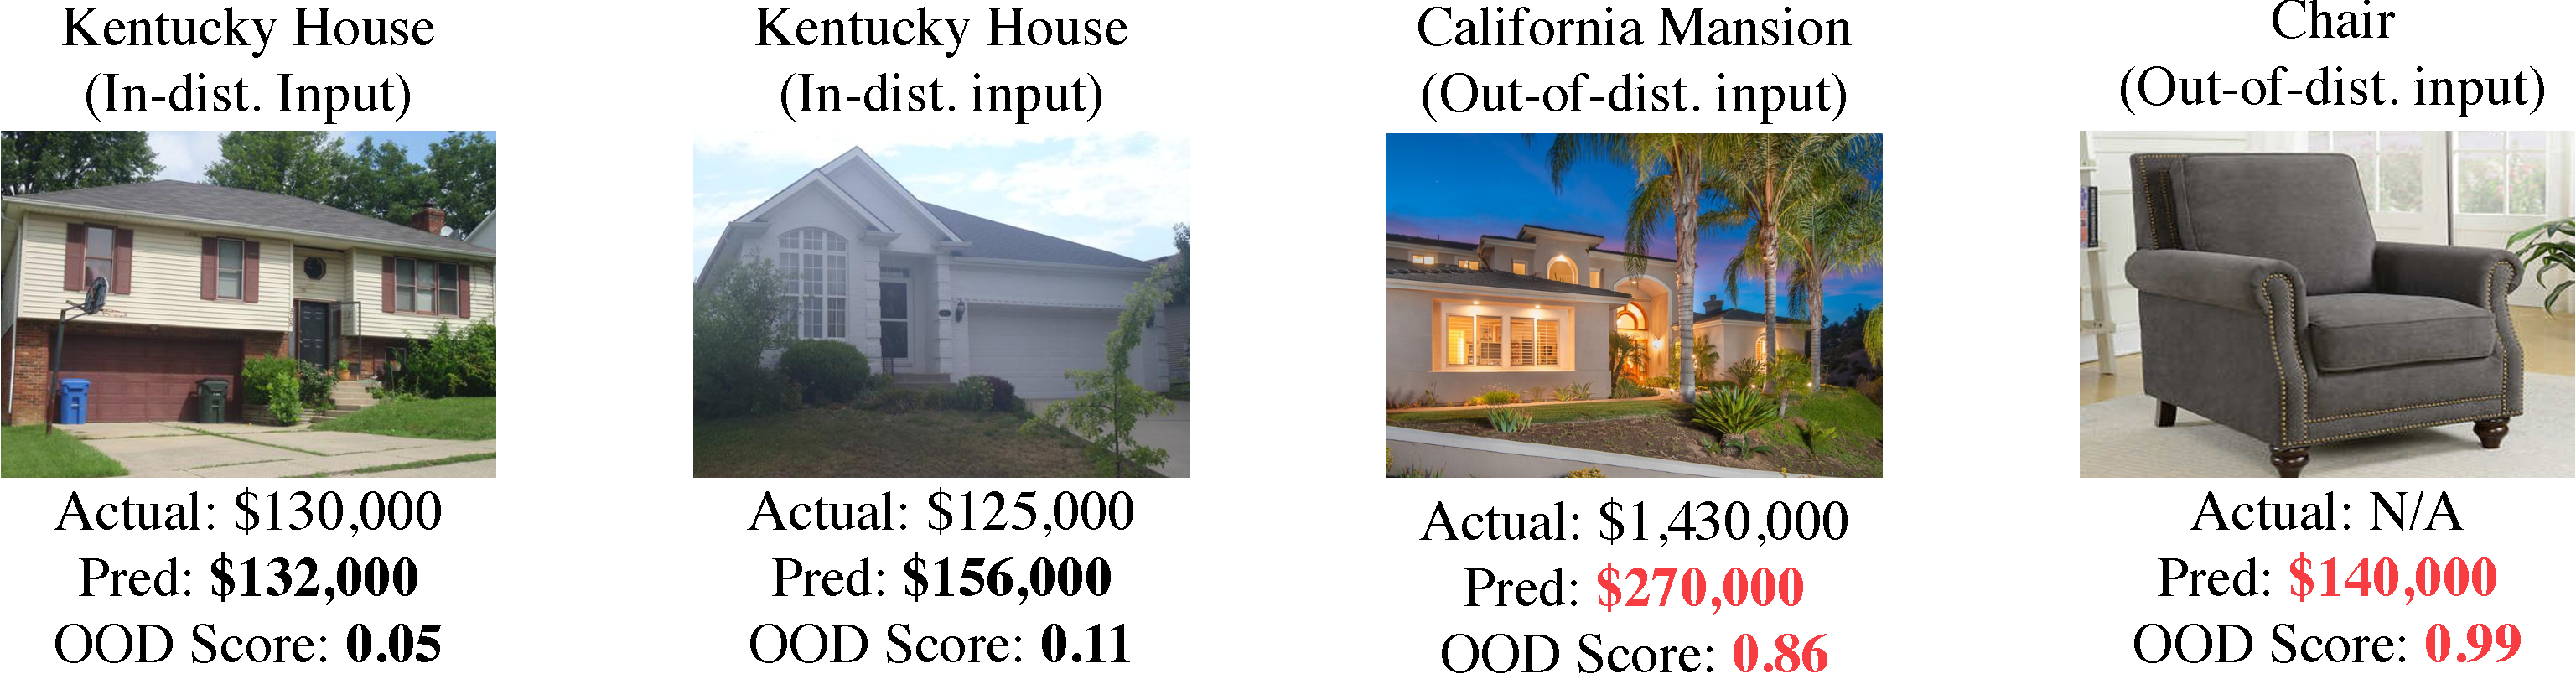
\includegraphics[width=\textwidth]{figures/ood_teaser.pdf}
  \caption{
    A neural network is trained to predict house prices in Kentucky.
    Although the algorithm generalizes well to in-distribution test images (left two houses),
    it has high error for the (out-of-distribution) mansion from California and makes a nonsensical prediction for the armchair.
    An ideal model would indicate that these predictions are anomolous/uncertain with an out-of-distribution (OOD) score.
  }
  \label{fig:ood_teaser}
\end{figure}

\paragraph{Preventing catastrophic failure.}

\paragraph{Improved predictive pipelines.}

\paragraph{Detecting anomalous inputs.}
Machine learning models will only generalize to data that are sufficiently similar to the training data.
If a model encounters \emph{out-of-distribution} (OOD) inputs -- inputs that deviate from the distribution of training data -- its predictions are likely to be erroneous or nonsensical \cite{begoli2019uncertainty,jiang2012calibrating}.
%This may occur if the model is used in scenarios that experience covariate shift \cite{sugiyama2007covariate} or if the model encounters previously-unseen categories of data \cite{yu2017occ,hassen2018openset}.
%Such scenarios are examples of \emph{out-of-distribution} (OOD) inputs.
This phenomenon is illustrated in \autoref{fig:ood_teaser}, which displays predictions from a neural network trained to predict prices of middle-class houses in Kentucky.
The model is able to make sensible predictions on other Kentucky houses (left and center-left images).
At the same time, the model vastly underestimates the price of a California mansion (center-right) and predicts and absurdly large price for a chair (right), as these inputs are not similar to any of the training set inputs.
This is because the range of predicted prices for the out-of-distribution matches the range of Kentucky housing prices.
A practitioner would see that the predictions are well within the model's expected output values and would be unaware that these predictions are nonsensical given the supplied inputs.

Well-modeled uncertainty estimates can to identify potentially anomalous data and prevent such erroneous predictions.
In this example, \gp{finish}

\paragraph{A principled exploration/exploitation tradeoff.}

\paragraph{Interpretability and trustworthiness.}
Good uncertainty estimates can provide a valuable extra bit of information to users of machine learning models when predictions may otherwise be difficult to interpret.
As machine learning algorithms become increasingly complex, they also appear more ``black box'' to users of such systems.
This presents several challenges, especially for models that are used to aid human decision makers in domains such as medicine, finance, and policy \gp{cite}.

For such circumstances it is therefore desirable for predictions to be understandable or interpretable \gp{cite LIME, saliency, etc.}.
There are many definitions for what constitutes a good ``explanation'' of black-box predictions, coming from policy makers \gp{cite gdpr, etc} and the research community \gp{cite} alike.
Though there are disagreements between these various sources, a well-calibrated uncertainty estimate is typically seen as a bare-minimum requirement for an interpretable prediction \gp{cite}.
Most humans -- even if they are unable to perform simple inferences \cite{gigerenzer2003simple} -- have natural intuition for interpreting confidence estimates as event-occurrence frequencies \cite{cosmides1996humans,hoffrage1998using}.
Therefore, well-calibrated confidence estimates from ML models can be easily interpreted by users.
Moreover, the presence of uncertainty estimates can affect a user's trust in a machine learning model.
In a study by \citet{zhou2017effects}, humans were asked to plan a budget for construction tasks based on information provided by a machine learning model.
Some participants received both predictions and confidence intervals from the machine learning model, while other users only received the predictions.
On tasks with low-to-moderate cognitive overhead, participants who saw uncertainty scores reported higher levels of trust in the machine learning model.

\section{Outline of Contributions}
